\subsection{Nguyên lý biến phân}

\begin{frame}{Biến phân khác gì với vi phân?}
    \vspace{-4mm}
    \begin{figure}
        \centering
        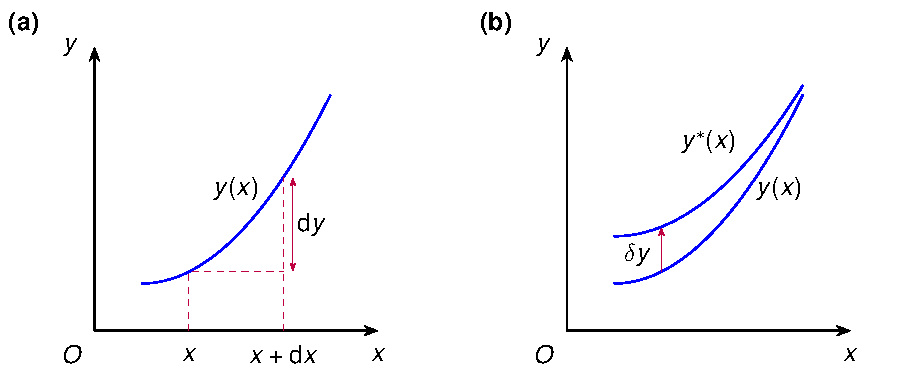
\includegraphics[width=\linewidth]{Figures/Variations.pdf}
        \caption{\textbf{(a)} Phép tính vi phân; \textbf{(b)} Phép tính biến phân. \cite{dao2002cohocgiaitich}}
        \label{fig:Variations}
    \end{figure}
\end{frame}


\subsection{Nguyên lý Maupertuis và nguyên lý Hamilton
về tác dụng tối thiểu}

\begin{frame}{Nguyên lý tác dụng tối thiểu và phương trình Euler}

\begin{columns}
\column{0.6\textwidth}
    \vspace{-3mm}
    \begin{itemize}
        \item Hàm tác dụng \( S \left[\mathbf{q}(t), \dot{\mathbf{q}}(t)\right] \) là tối thiểu.
    \end{itemize}
    \begin{equation}
        S \left[\mathbf{q}(t), \dot{\mathbf{q}}(t)\right] = \int_{t_1}^{t_2} L\left[ \mathbf{q}(t), \dot{\mathbf{q}}(t), t \right] \mathrm{d}t,
    \end{equation}

    \begin{equation} \label{eq:deltaS}
        \delta S = \int_{t_1}^{t_2} \left( \frac{\partial L}{\partial \mathbf{q}} \delta \mathbf{q} + \frac{\partial L}{\partial \dot{\mathbf{q}}} \delta \dot{\mathbf{q}} \right) \mathrm{d}t.
    \end{equation}

    Định lý Leibnitz cho biến phân \(\delta \dot{\mathbf{q}} = \mathrm{d}\left( \delta \mathbf{q} \right) / \mathrm{d}t\)

    \begin{equation}
        \delta S = \int_{t_1}^{t_2} \left( \frac{\partial L}{\partial \mathbf{q}} - \frac{\mathrm{d}}{\mathrm{d}t} \left( \frac{\partial L}{\partial \dot{\mathbf{q}}} \right) \right) \delta \mathbf{q} \mathrm{d}t + \left[ \frac{\partial L}{\partial \dot{\mathbf{q}}} \delta \mathbf{q} \right] \Big|_{t_1}^{t_2}.
    \end{equation}

\column{0.4\textwidth}
    Hàm tác dụng \(S\) đạt cực tiểu khi \(\mathbf{q}(t)\) thỏa mãn phương trình
    \begin{equation}
        \frac{\partial L}{\partial \mathbf{q}} - \frac{\mathrm{d}}{\mathrm{d}t} \left( \frac{\partial L}{\partial \dot{\mathbf{q}}} \right) = 0.
    \end{equation}

    % \begin{itemize}
    %     \item \(L = T - U\) trong cơ học cổ điển.
    %     \item \(L = m c^2 \sqrt{1 - \frac{v^2}{c^2}} \) trong cơ học tương đối tính.
    % \end{itemize}

    \begin{itemize}
        \item Tích phân Euler
    \end{itemize}
    \begin{equation}
        \dfrac{\partial L}{\partial t} + \dfrac{\mathrm{d} }{\mathrm{d} t} \left( \dot{\mathbf{q}} \dfrac{\partial L}{\partial \dot{\mathbf{q}}} - L \right) = 0.
    \end{equation}
    Khi \(\partial L/\partial t = 0\) thì
    \begin{equation}
        H = \dot{\mathbf{q}} \dfrac{\partial L}{\partial \dot{\mathbf{q}}} - L = \text{const}.
    \end{equation}
\end{columns}
    
\end{frame}


\subsection{Các ứng dụng của nguyên lý tác dụng tối thiểu trong vật lý}

\begin{frame}{Catenary - Cực tiểu thế năng trong tĩnh học}
\begin{columns}
\column{0.5\textwidth}
    Thế năng trọng trường của dây xích
    \begin{equation}
        U = \int y \lambda g \sqrt{ y'^2(x) + 1} \mathrm{d} x.
    \end{equation}
    Nên Lagrangian của hệ
    \begin{equation}
        L = \lambda g y \sqrt{ y'^2(x) + 1}
    \end{equation}
    Giải phương trình Euler\footnote{Hoặc tích phân Euler \cite{cline2017variational}.}, ta được
    \begin{equation}
        y = A \cosh \left( \frac{x}{A} \right).
    \end{equation}
    
\column{0.5\textwidth}
    \vspace{-5mm}
    \begin{figure}
        \centering
        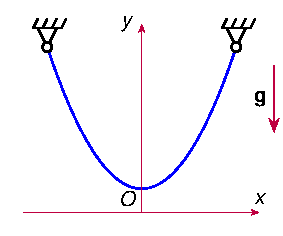
\includegraphics[width=0.9\linewidth]{Figures/Catenary.pdf}
        \caption{Đường Catenary của một dây xích cố định hai đầu đặt trong trọng trường.}
        \label{fig:Catenary}
    \end{figure}
\end{columns}
\end{frame}


\begin{frame}{Nguyên lý Fermat trong quang hình học}

\begin{columns}
\column{0.5\textwidth}
    Thời gian ánh sáng truyền từ \(A\) đến \(B\)
    \begin{equation}
        t = \int_A^B \frac{n}{c} \mathrm{d}s = \frac{1}{c} \int_A^B n(x) \sqrt{1 + y'^2(x)} \mathrm{d}x.
    \end{equation}
    Nên Lagrangian của hệ
    \begin{equation}
        L = n(x) \sqrt{1 + y'^2(x)}.
    \end{equation}
    Giải phương trình Euler, ta được
    \begin{equation}
        n(x) \frac{y'}{\sqrt{1 + y'^2}} = \text{const}.
    \end{equation}
\column{0.5\textwidth}
    \vspace{-9mm}
    \begin{figure}
        \centering
        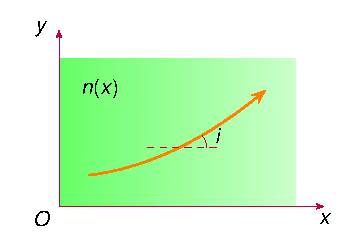
\includegraphics[width=0.9\linewidth]{Figures/Gradient_index.pdf}
        \caption{Ánh sáng truyền trong môi trường có chiết suất biến thiên theo vị trí.}
        \label{fig:Gradient_index}
    \end{figure}
    \vspace{-4mm}
    \begin{itemize}
        \item \(n(x) \sin (i) = \text{const}\) (định luật Snell).
    \end{itemize}
\end{columns}


\end{frame}
